\chapter{The CMS Experiment at the Large Hadron Collider}
\section{Introduction}
The Large Hadron Collider (LHC) is a proton-proton ($\Pp\Pp$) accelerator
located at the CERN particle physics laboratory near Geneva, Switzerland. The
LHC is built in the tunnels formerly occupied by the LEP experiment, a
\unit{27}{\kilo\metre} long ring lying on the border between France and Switzerland. Two
beams of protons run in opposite directions around the ring and are made to
collide at four interaction points.

There are four primary experiments at the LHC: \ac{ALICE}, \ac{ATLAS}, \ac{CMS}
and \ac{LHCb}. Each one is constructed around one of the four interaction points
and records the shower of particles produced from the colliding protons. ATLAS
and CMS are large, general purpose detectors designed to search for a variety of
\ac{NP} signatures as well as making higher precision measurements of \ac{SM}
parameters. \ac{ALICE} is designed to examine the products of heavy-ion
collisions (lead-lead) in order to explore the quark gluon plasma and related
physics. Finally, the \ac{LHCb} experiment is optimised for the study of B-meson
decays. These are important for the study of CP violation within the \ac{SM} but
might also provide potential avenues for the discovery of \ac{NP}.

In addition to the four larger detectors, two smaller experiments, \ac{LHCf} and
\ac{TOTEM} lie upstream of the \ac{ATLAS} and \ac{CMS} collision points in order
to probe more specialised forward physics phenomena.

\section{The \acl{LHC}}
The \ac{LHC} is a circular $\Pp\Pp$ synchrotron with a circumference of
\unit{27}{km}. It sits in a tunnel initially constructed for the \ac{LEP}
accelerator buried at a depth of between 50 and \unit{175}{\metre} beneath the
Franco-Swiss border. At full design specifications, 2808 bunches of protons will
circulate around each direction of the ring, colliding at a centre of mass
energy of \unit{14}{\TeV}. With a proton bunch spacing of
\unit{25}{\ns}, the \ac{LHC} will eventually achieve a luminosity of
\unit{$10^{34}$}{\rpsquare{\centi\metre}\usk\reciprocal\second}.

\subsection{Accelerator Complex}
The \ac{LHC} ring itself is the final stage in an injector chain utilising a
series of accelerators built at CERN over the last 50 years. Each stage supplies
an incremental increase in the proton (or heavy ion) bunch energy. The first
stage in this chain is a linear accelerator, either the Linac2 for proton
injection or Linac3 during heavy-ion runs. The Linac2 injects protons into the
\ac{PSB} at an energy of \unit{50}{\mega\electronvolt}. Similarly, the ions
proceed first from the Linac3 to the \ac{LEIR} before finally arriving at the
\ac{PS}. From here on, the paths of the protons and heavy-ions are the
same. Proton bunches pass from the \ac{PSB} to the \ac{PS} at an energy of
\unit{1.4}{\giga\electronvolt} and then on to the \ac{SPS} at an energy of
\unit{28}{\giga\electronvolt}. Protons then arrive at the \ac{SPS}, where they
circulate around a ring \unit{2}{\kilo\metre} in diameter, and increasing their
energy to \unit{450}{\giga\electronvolt}. From here, kicker magnets inject the
bunches into the \ac{LHC} itself, where the energy is finally increased to the
design specified \unit{7}{\TeV} per beam.
\begin{figure}
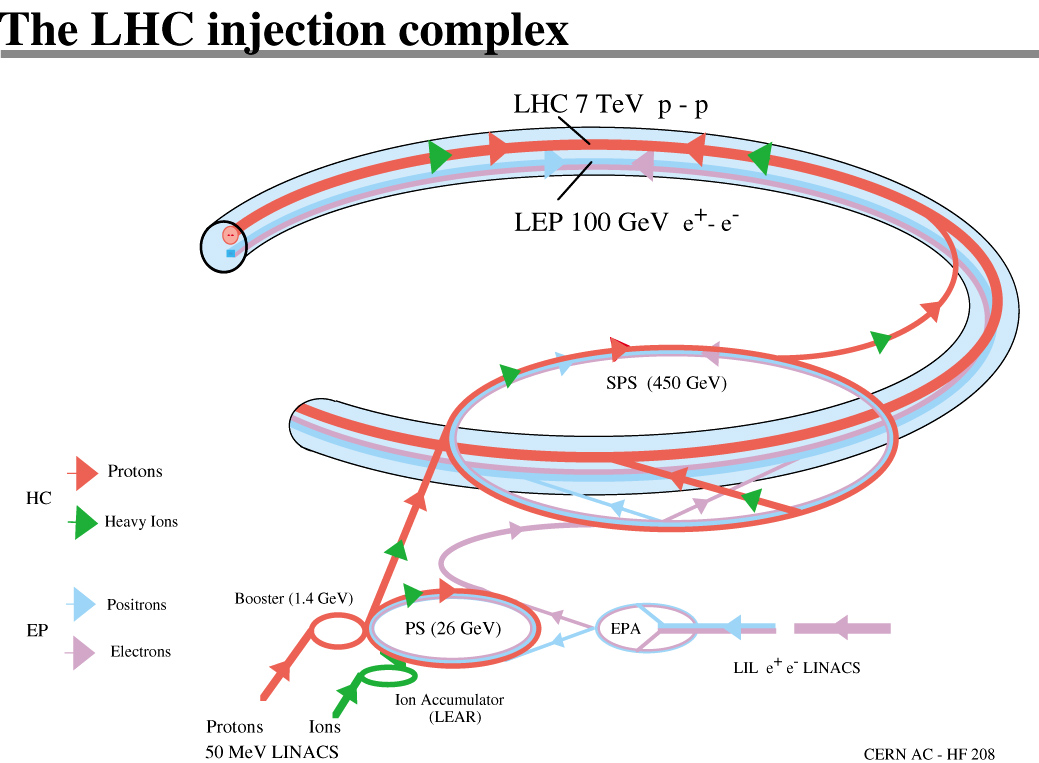
\includegraphics[width=0.9\textwidth]{fig/lhc-pho-1993-008}
\end{figure}

\ctable[
cap=LHC Accelerator Complex,
caption=LHC Accelerator Complex,
mincapwidth=0.5\textwidth,
pos=h
]{lcc}{
\tnote[a]{Heavy-Ions only}
}{\FL
Accelerator & Energy \ML
%
Linac2   & \unit{50}{\mega\electronvolt} \NN
Linac3\tmark[a]   & \unit{4.2}{\mega\electronvolt\per u} \ML
%
\acf{PSB} & \unit{1.4}{\giga\electronvolt} \NN
\acf{LEIR}\tmark[a]   & \unit{??}{\mega\electronvolt\per u} \ML
%
\acf{PS} & \unit{28}{\giga\electronvolt} \NN
\acf{SPS} & \unit{450}{\giga\electronvolt} \NN
\acf{LHC} & \unit{7}{\tera\electronvolt} \LL
}


\section{The \acl{CMS} Experiment}
\ac{CMS} is a large, general purpose detector designed to firmly establish or
disprove the existence of the Higgs boson particle as well as performing
searches for a wide variety of \ac{NP} signatures. The design goals of CMS were
as follows (paraphrasing Design proposal):
\begin{enumerate}
\item a high quality, redundant muon system,
\item the best possible \ac{ECAL}
\item high quality central tracking to complement these two systems
\item an affordable detector
\end{enumerate}

These goals motivated the design of a traditional cylindrical detector,
\unit{21.5}{\metre} in length and \unit{15}{\metre} in diameter. A key feature
of the design is the \unit{4}{\tesla} superconducting solenoid. The bending
field supplied provides accurate muon momentum resolution up to energies of
\unit{$\approx$ 1}{\TeV}. The size of the solenoid placed stringent
limitations on the volume of the inner detector subsystems (everything except
for the muon chambers and return yoke).

\subsection{Coordinate System}
The \ac{CMS} coordinate system

\subsection{Silicon Tracker}
The innermost subsystem of \ac{CMS} is the silicon tracker, designed to provide
highly precise measurements of particle trajectories close to the CMS
interaction point. The tracker extends to pseudorapidities of $|\eta|<2.5$ and
has an active silicon area of more than \unit{200}{\metre\squared} making it the
largest silicon tracker ever built.

The tracker design can be better understood by considering the expected particle
flux at design luminosity as a function of radial distance $r$ from the
beamline.

\begin{itemize}
\item At $ r \approx \unit{10}{\cm}$ the particle flux is highest. Accordingly,
  the innermost layer of the CMS tracker is comprised of hybrid pixels. With an
  area of \unit{$100\times 150$}{\micro\metre\squared}, particle densities are
  $O(10^{-4})$ per pixel per LHC bunch crossing.
\item At a radius \unit{$20 < r < 55$}{\centi\metre}, reduced particle flux allows
  the use of silicon microstrip sensors. With a much larger area of
  $\unit{10}{\centi\metre}\times\unit{80}{\micro\metre}$, average particle
  densities are $O(10^{-2})$ per strip per bunch crossing.
 \item At $ r > \unit{55}{\cm}$, the silicon strip size is once again increased
   to $\unit{25}{\cm}\times \unit{180}{\cm}$ again giving a particle density of
   $O(10^{-2})$ per strip per bunch crossing.
\end{itemize}

\subsubsection{Pixel Tracker}
The hybrid pixels are placed closest to the interaction point. As well as
maintaining an acceptable particle density per sensor, their close proximity to
the interaction point allows the origin of collision products to be accurately
determined. This is of particular importance for instance in B-tagging. In the
barrel region, 3 layers are placed at mean radii of 4.4, 7.3 and
\unit{10.2}{\cm}. The detector has a length of \unit{53}{\cm} in the $z$
direction. The end discs are instrumented with only two layers and are located
at $|z|=34.5, \unit{46.5}{\cm}$. The pixel modules in these layers are arranged
in a turbine-like layout.

To acheive the desired spatial resolution, the pixels have an almost square
geometry with an area of \unit{$150\times 100$}{\micro\metre\squared} in the
$r\phi\times z$ ($r\times r\phi$) for the barrel (end discs).

\subsubsection{Strip Tracker}
Further from the interaction point, the tracker is instrumented with silicon
strip detectors. The barrel component can be further divided into the \ac{TIB}
and the \ac{TOB}. The \ac{TIB} is composed of 4 layers with the \ac{TOB}
comprising a further 6. The \ac{TOB} extends to $z = \pm
\unit{118}{\centi\metre}$. Beyond this are the endcaps which can again be split
into two components: the \ac{TEC} made up of 9 disks and the \ac{TID} 3. The
silicon micro strip sensors are \unit{320}{\micro\metre} thick and oriented
parallel to the $z$ axis in the barrel and radially in the disks.

Both the \ac{TIB} and \ac{TID} supply up to four measurements of $r\phi$. With a
strip-pitch of \unit{80}{\micro\metre} in the inner two layers and
\unit{120}{\micro\metre} in the outer two, the \ac{TIB} achieves a single point
resolution of \unit{23 and 35}{\micro\metre} respectively. In the \ac{TID}, the
strip pitch varies between \unit{100 and 141}{\micro\metre}.

The \ac{TOB} uses \unit{500}{\micro\metre} thick sensors with a strip-pitch of
\unit{183}{\micro\metre} in the first four layers and \unit{122}{\micro\metre} in
the outer two. This gives a single point resolution of \unit{53}{\micro\metre}
and \unit{35}{\micro\metre} respectively.

The first two layers of the \ac{TIB}, \ac{TOB} and \ac{TID} and rings 1, 2 and 5
of the \ac{TEC} are so-called stereo modules. These are double-sided modules
where the two layers of strips have a stereo angle of \unit{100}{\milli\radian}
between them. This provides additional resolution in the $z$ measurement in the
barrel (or $r$ in the endcaps). The resolution of this measurement is
\unit{230}{\micro\metre} and \unit{530}{\micro\metre} in the \ac{TIB} and
\ac{TOB} respectively.

\begin{figure}
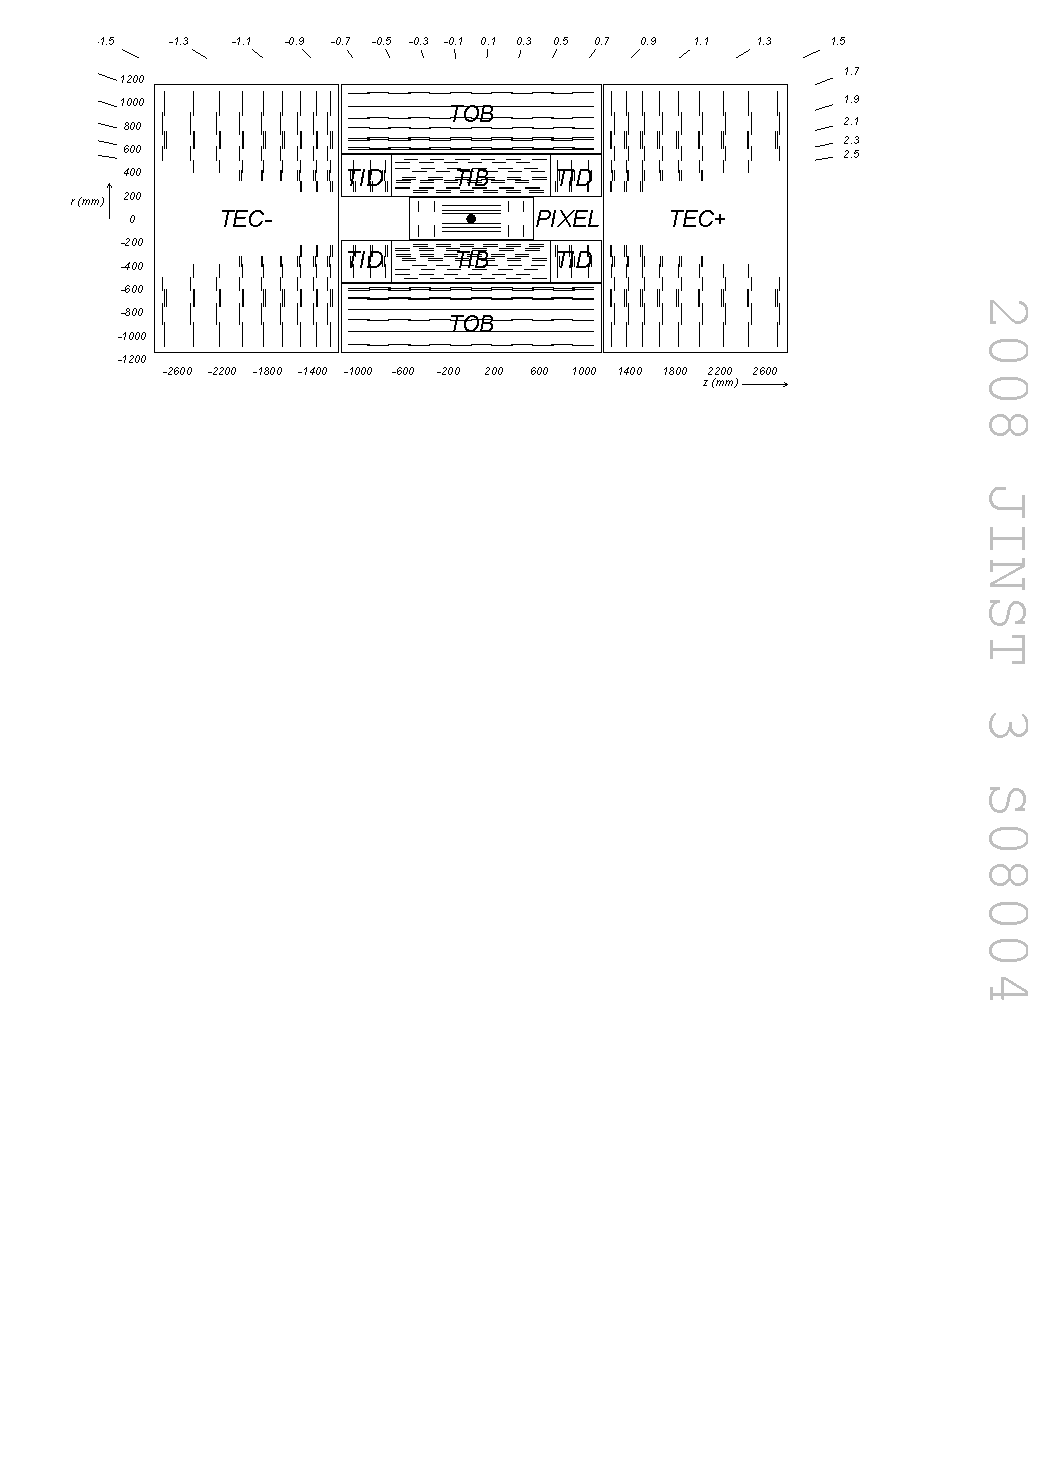
\includegraphics[width=\textwidth]{fig/tracker}
\end{figure}

\subsection{\acl{ECAL}}
The \ac{ECAL} surrounds the silicon tracker and provides a high resolution
measurement of electromagnetic showers within a homogeneous, hermetic
calorimeter composed of 61,200 lead tungstate (PbWO$_4$) crystals. This material
was chosen for its high desnity, short radiation length and small Moli\`{e}re
radius. Scintillation photons are then recorded by \ac{APD}s in the barrel and
\ac{VPT}s in the endcap. The driving motivation for the \ac{ECAL} design was the
detection of the low-mass favoured Higgs decay channel
$PH\longrightarrow\gamma\gamma$.

\subsubsection{\acl{EB}}
The \ac{EB} extends in rapidity to $|\eta|<1.479|$ with a crystal
segmentation of $360\times 85$ ($\eta-\phi$) in each half barrel. Each crystal
is slightly tapered with a cross-section of $0.0174\times0.0174$ in
$\eta-phi$. The crystals have a front cross section of \unit{$22\times
  22$}{\milli\metre\squared} and a length of \unit{230}{\milli\metre}
(corresponding to 25.8 radiation lengths).

\subsubsection{\acl{EE}}
The \ac{EE} occupies the rapidity range $1.479 < |\eta| < 3.0$. Crystals are
grouped into $5\times 5$ supercrystals within a carbon-fibre alveolar
structure. The endcaps are split into two halves, known as Dees, each holding
3,662 crystals.

The scintillation of the ac{ECAL} crystals as well as the amplification of the
\ac{APDs} varies as a function of temperature. This variation was found to be
\unit{$\approx 4\%$}{\per\celsius}. For this reason, the \ac{ECAL} temperature
is precisely regulated to within \unit{$\pm$ 0.05}{\celsius}.

\subsection{\acl{HCAL}}
Accurate measurement of hadronic showers is crucial for analyses involving jets
or missing energy type signatures. The \ac{HCAL} lies between the outer edge of
the ECAL and the inner edge of the solenoid ($\unit{1.77}{\metre} < r <
\unit{2.95}{\metre}$). This constrains the size of the \ac{HCAL} to a relatively
compact design and necessitates the placement of a ``tail catcher'' outside of
the solenoid.

\subsubsection{\acl{HB}}
\subsubsection{\acl{HE}}


\subsection{Magnet}
\subsection{Muon Chambers}
As has already been said, sensitive detection of muons is one of \ac{CMS}'s key
design goals. Since the effect of radiative losses in the tracker is much less
for muons than it is for electrons, muons are able to provide a much finer mass
resolution which can be used in a variety of physics searches and
measurements. The muon system at CMS is responsible for muon identification,
momentum measurement and triggering (for further detail see
Section~\ref{sec:trigger}). Three types of detectors are used, chosen for
different regions of the detector according to the magnetic field level, muon
rate and response time required for input to the trigger.

\subsubsection{Drift Tubes}


\subsection{Data Aquisition and Trigger System}
